\documentclass[basic]{inVerba-notes}
\usepackage{inVerba-math}
% chktex-file 3
\newcommand{\userName}{Cullyn Newman}
\newcommand{\class}{MTH:\@ 261}
\newcommand{\theTitle}{Transform Yourself}
\newcommand{\institution}{Portland State University}

\newcommand{\N}{\mathbb{N}}
\newcommand{\Z}{\mathbb{Z}}
\newcommand{\Q}{\mathbb{Q}}
\newcommand{\R}{\mathbb{R}}
\newcommand{\A}{\mathbb{A}}

\begin{document}
\begin{enumerate}[align=left, leftmargin=0pt, labelindent=\parindent, listparindent=\parindent, labelwidth=0pt, itemindent=!]\color{minor}

  \item Let \(A = \begin{bmatrix*}[r] -1 & 0 \\ 0 & -1 \end{bmatrix*}\) and define a transformation  \(S: \R^2 \to \R^2\) by \(S(\bm{x}) = A\bm{x}\). Describe in a sentence what \(S \) does.
  
  \basec{\begin{itemize}
    \item \(S\) is a transformation that takes any vector \(\bm{x}\) in \(\mathbb{R}^2\) and scales it by \(-1\). Scaling by negative -1 simply inverts the direction, or in other words, \(S\) is a reflection through both the \(x\) and \(y\) axes.
  \end{itemize}}
  
  \bigskip

  \item Let \(T: \R^2 \to \R^2\) be the transformation that expands the plane by a factor of 1.5 in all directions (that is, all entries in the vector grow by a factor of 1.5; see below). Define a matrix \(B\) so that \(T(\bm{x}) = B\bm{x}\).

  \begin{multicols}{2}
  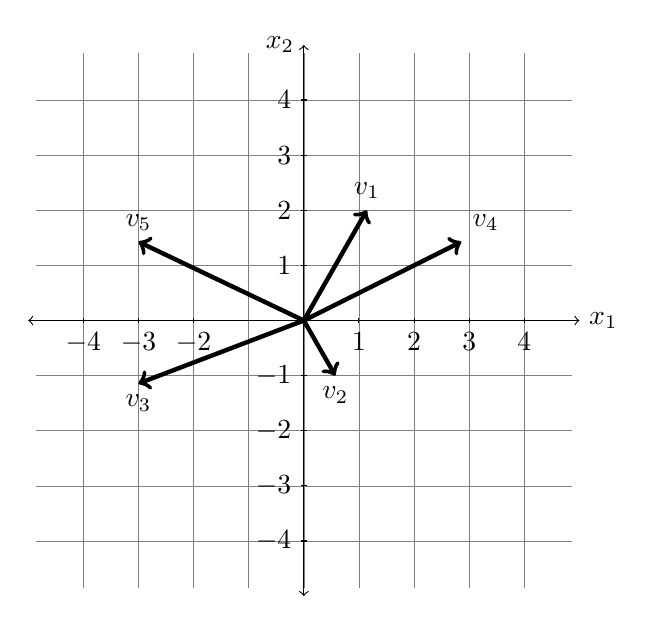
\begin{tikzpicture}
  %grid
  \draw[step=.7cm, very thin,color=gray] (-3.4,-3.4) grid (3.4,3.4);
  \draw[<->] (-3.5,0) -- (3.5,0) node[right] {$x_1$};
  \draw[<->] (0,-3.5) -- (0,3.5) node[left] {$x_2$};
  \foreach \x in {-4, -3, -2,1,2,3,4}
  \draw (.7*\x cm,1pt) -- (.7*\x cm,-1pt) node[anchor=north] {$\x$};
  \foreach \y in { -4, -3, -2, -1,1,2,3,4}
  \draw (1pt, .7*\y cm) -- (-1pt, .7*\y cm) node[anchor=east] {$\y$};
  %vectors
  \draw[ultra thick, ->] (0,0) -- (.8, 1.4) node[anchor=south] {$\bm{v}_1$};
  \draw[ultra thick, ->] (0,0) -- (.4, -.7) node[anchor=north] {$\bm{v}_2$};
  \draw[ultra thick, ->] (0,0) -- (-2.1, -.8) node[anchor=north] {$\bm{v}_3$};
  \draw[ultra thick, ->] (0,0) -- (2, 1) node[anchor=south west] {$\bm{v}_4$};
  \draw[ultra thick, ->] (0,0) -- (-2.1, 1) node[anchor=south] {$\bm{v}_5$};
  \end{tikzpicture}
  
  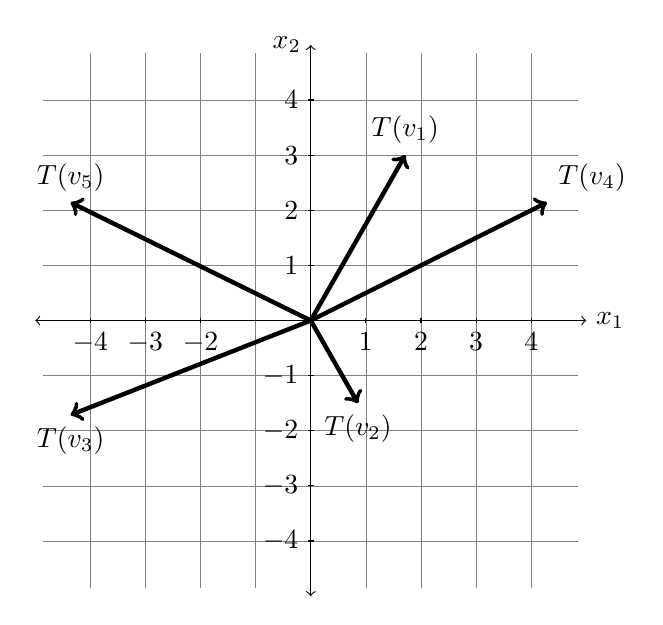
\begin{tikzpicture}
  %grid
  \draw[step=.7cm, very thin,color=gray] (-3.4,-3.4) grid (3.4,3.4);
  \draw[<->] (-3.5,0) -- (3.5,0) node[right] {$x_1$};
  \draw[<->] (0,-3.5) -- (0,3.5) node[left] {$x_2$};
  \foreach \x in {-4, -3, -2, 1,2,3,4}
  \draw (.7*\x cm,1pt) -- (.7*\x cm,-1pt) node[anchor=north] {$\x$};
  \foreach \y in { -4, -3, -2, -1,1,2,3,4}
  \draw (1pt, .7*\y cm) -- (-1pt, .7*\y cm) node[anchor=east] {$\y$};
  %vectors
  \draw[ultra thick, ->] (0,0) -- (1.2, 2.1) node[anchor=south] {$T(\bm{v}_1)$};
  \draw[ultra thick, ->] (0,0) -- (.6, -1.05) node[anchor=north] {$T(\bm{v}_2)$};
  \draw[ultra thick, ->] (0,0) -- (-3.05, -1.2) node[anchor=north] {$T(\bm{v}_3)$};
  \draw[ultra thick, ->] (0,0) -- (3, 1.5) node[anchor=south west] {$T(\bm{v}_4)$};
  \draw[ultra thick, ->] (0,0) -- (-3.05, 1.5) node[anchor=south] {$T(\bm{v}_5)$};
  \end{tikzpicture}
  \end{multicols}
  
  \basec{\[%%%%%%%%%%%%%%%%%%%%%%%%%%%%%%%%%%%%%%%%%%%%%%%
  \bm{B} = 1.5 \bm{I} = \begin{bmatrix}
  1.5 & 0 \\
  0 & 1.5 
  \end{bmatrix}
  \]}%%%%%%%%%%%%%%%%%%%%%%%%%%%%%%%%%%%%%%%%%%%%%%%%%%%%%%
  
\end{enumerate}

\end{document}